\documentclass{article}

% if you need to pass options to natbib, use, e.g.:
%     \PassOptionsToPackage{numbers, compress}{natbib}
% before loading neurips_2023

% ready for submission
\usepackage[final]{neurips_2023}

% to avoid loading the natbib package, add option nonatbib:
%    \usepackage[nonatbib]{neurips_2023}


\usepackage[utf8]{inputenc} % allow utf-8 input
\usepackage[T1]{fontenc}    % use 8-bit T1 fonts
\usepackage{hyperref}       % hyperlinks
\usepackage{url}            % simple URL typesetting
\usepackage{booktabs}       % professional-quality tables
\usepackage{amsfonts}       % blackboard math symbols
\usepackage{nicefrac}       % compact symbols for 1/2, etc.
\usepackage{microtype}      % microtypography
\usepackage{xcolor}         % colors


\usepackage{graphicx}
\usepackage[font=small,skip=2pt]{caption}

\usepackage{lipsum}         % placeholder text generation
\usepackage{subcaption} 


% Damit die (sub)sections wie in der angabe formatiert sind: 1.), ..., a.), ...
\renewcommand{\thesection}{\arabic{section}.)}
\renewcommand{\thesubsection}{\alph{subsection}.)}


\title{MLPC Report  - Task 4: Challenge}


% The \author macro works with any number of authors. There are two commands
% used to separate the names and addresses of multiple authors: \And and \AND.
%
% Using \And between authors leaves it to LaTeX to determine where to break the
% lines. Using \AND forces a line break at that point. So, if LaTeX puts 3 of 4
% authors names on the first line, and the last on the second line, try using
% \AND instead of \And before the third author name.


% Sorry, musste die Namen alphabetisch anordnen, hätte mich sonst zu sehr getriggered :(
% Kein Problem die Anordnung war wie die Gruppen Liste im Moodle ist.

\author{
  Team OBSERVE \AND
  Johannes Grafinger 
  \And
  Jonas Gantar 
  \And 
  Leonhard Markus Spanring 
  \And 
  Reinhard Josef Pötscher
}

\begin{document}

\maketitle

\begin{contributions}
  \textcolor{blue}{All of us together were responsible for tasks 1.) and 2.) .} 
  \textcolor{magenta}{All of us together were responsible for tasks 3.) and 4.) .} 
  \textcolor{red}{All of us together were responsible for task 5.) Bonus.} 
  In the same constellation we created this report. We all worked on the presentation together, with Group 2 providing its content. We held regular meetings, where each group presented their results up to that point and the other critically reviewing their work.
  \textcolor{green}{Collaboration was done over GitHub and project progression was tracked through regular stand-ups.} 
\end{contributions}


\section{Describe your evaluation setup}
\label{sec:Describe your evaluation setup}




\subsection{How did you split the development dataset (provided in phase three of the project) into a training and evaluation set while avoiding information leakage?}
\label{sec:Describe:a}




\subsection{Establish and describe a naive baseline system (i.e., a baseline without a classifier). How much cost can we expect from it?}
\label{sec:Describe:b}





\newpage


\section{Build a simple SED system, that predicts the presence and absence of the ten sound categories in 1.2-second audio segments.} 
\label{sec:Build a simple SED system}

Our starting point for a simple SED system is a Temporal Convolutional Network (TCN) architecture. We chose this architecture specifically for several reasons:
\newline
Unlike Recurrent Neural Networks (RNNs), assuming proper dilation settings, they can model long-term dependencies much more efficiently than RNNs, without needing to resort to recursion. They do not rely on sequential processing, which generally makes them much faster to train and easier to parallelize. They are relatively light-weight architectures, especially when compared to transformer based methods. This also makes them less likely to overfit, which we believe might become problem with some of the rarer classes.

Our network takes in the whole F$\times$D array of an audio file, with F representing the number of frames, and D the number of feature (audio embedding) dimensions. The output of the model is then of shape F$\times$10, one probability for each class per frame.

A more detailed description of our architecture: The input is first passed through a Convolutional Feature Extractor block, whose main job is to downsample the D input features into a more compact representation useful for predicting the different classes. In our case, we end up with a F$\times$128 array. For our actual TCN, we then use 4 residual blocks, with dilations of $2^0, \dots, 2^3$ and kernel size of 3. Throughout our model, we also added several BatchNorm and Dropout layers. A more detailed description can be seen in \hyperref[tab:architecture]{Table \ref{tab:architecture}}.

\begin{table}[h]
\centering
\begin{adjustbox}{width=\textwidth}
\begin{tabular}{|c|c|c|c|}
\hline
\textbf{Layer} & \textbf{Input Shape} & \textbf{Output Shape} & \textbf{Details} \\
\hline
\multicolumn{4}{|c|}{\textbf{Convolutional Feature Extractor}} \\
\hline
Input & $[B, F, D]$ & $[B, F, D]$ & Raw frame-level features \\
\hline
Transpose & $[B, D, F]$ & $[B, D, F]$ & Prepare for Conv1D over embedding axis \\
\hline
Conv1D + BN + ReLU & $[B, D, F]$ & $[B, C, F]$ & $1^{\text{st}}$ Conv1D block, kernel size = 3, padding = 1 \\
\hline
Dropout & $[B, C, F]$ & $[B, C, F]$ & Dropout rate = 0.2 \\
\hline
Conv1D + BN + ReLU & $[B, C, F]$ & $[B, C, F]$ & $2^{\text{nd}}$ Conv1D block, kernel size = 3, padding = 1 \\
\hline
\multicolumn{4}{|c|}{\textbf{TCN (Temporal Convolutional Network)}} \\
\hline
ResidualBlock (× num\_blocks) & $[B, C, T]$ & $[B, C, T]$ & Each block: 2 × Conv1D + BN + ReLU + Dropout = 0.2, dilations = $2^i$ \\
\hline
Conv1D (output layer) & $[B, C, T]$ & $[B, N, T]$ & Kernel size = 1 \\
\hline
Transpose & $[B, N, T]$ & $[B, T, N]$ & Final output for framewise classification \\
\hline
\end{tabular}
\end{adjustbox}
\captionsetup{justification=centering}
\caption{Architecture of our network, \\ B: BatchSize, F: Number of Frames, D: Input Dimensionality, C: Reduced Dimensionality, N: Number of Classes}
\label{tab:architecture}
\end{table}

Our model is trained on the training data. After each epoch, it's performance on the validation data is recorded to keep track of and save the best version of the model. We use Binary Cross Entropy as our loss function, a batch size of 64, a learning rate of 1e-4 as well as the Adam optimizer (these setting were kept from the tutorial notebook).

We want to take a moment to point out that our model is pretty lightweight with around 750K parameters, especially when compared to something like the BiGRU used in the tutorial, which has around 20 Million and performs worse. This is of course not part of the task, but noteworthy anyways and should be considered when implementing a system like this.

\subsection{How did you threshold and combine predictions to derive a label for the 1.2-second segments? Describe any heuristics or post-processing strategies used.}
\label{sec:Build:a}
Of course, frame wise probabilities for each class are not enough to classify something. In order to actually predict if a class is present within a given frame we need to binarize our predictions by thresholding them. For now, we decided to use a simple constant threshold value of 0.5 for this.
\newline
Then there is the problem of combining the predictions made for all frames into ones for 1.2 second-segments. Since our hop length is 120ms, 10 frames correspond to 1.2 seconds. Our simple aggregation strategy now is the following: If a class is active within at least one of these 10 frames, the class is said to be active within the segment, otherwise it is labeled as inactive. Since this is in line with how the actual labels are computed, we decided that it most likely would not make a lot of sense to do something different.


\subsection{What strategies did you apply to minimize the task-specific cost function?}
\label{sec:Build:b}
In order to minimize our task specific cost function, which assigns different costs to False Negatives (FN) and False Positives (FP) for each class, we created a custom Binary-Cross-Entropy (BCE) Loss function. It computes the regular BCE Loss for each class, and then by looking at the targets, scales each entry by either it's FP (if the target is 1) or FN (if the target is 0) cost. Doing this improved performance by quite a bit.
\newline
Using this custom loss already lowered the lowest cost on the validation data from 43.17488 to 40.1256.




\subsection{Does your classifier-based SED system achieve lower costs compared to the naive baseline system you established in step 1? If not, describe possible issues.}
\label{sec:Build:c}
Yes, our simple SED system does outperform the naive baseline by quit a bit when it comes to our specific cost function (and likely most other metrics as well). This is not really impressive however, as the costs for False Negatives are higher than for False Positives, so most methods which at least sometimes predict a positive label should perform better.
\newline
In the current state, our SED system achieves a total average cost of about 40.1256 on the validation data.

\newpage


\section{Investigate at least three diverse strategies to improve your starting point}
\label{sec:Investigate diverse strategies}




\subsection{For each of these strategies: Describe the main ideas you had and hypotheses you tried, as well as their outcome after experimentally verifying or falsifying the hypotheses (via validation on (parts of) the development set). Do not hesitate to report negative outcomes.}
\label{sec:Investigate:a}

\textbf{Strategy 1: Using variable thresholds for the different classes}
\newline
Using a simple globally constant threshold for each class does work (as has been shown in \hyperref[sec:Build a simple SED system]{2.)} ), but most likely is not optimal. Factors like the heavy class imbalances or the models sensitivity to the different classes are completely ignored this way. Additionally, the different costs associated with each class also are not accounted for.
\newline
For this reason, we wanted to tune the thresholds for each of the 10 classes as well. For each class, our threshold search space consists of values from 0 to 1, in intervals of 0.05. After each validation epoch, we tune the thresholds for each class by picking the one which maximises the following utility function: $U = TP - cost_{FP}FP - cost_{FN}FN$.

\textbf{Strategy 2: Post-processing model outputs before aggregation}
\newline
Considering our aggregation strategy discussed in \hyperref[sec:Build:a]{2.) a.)}, spurious positive class predictions lasting only a few frames could potentially have a big effect on overall performance. This might even be amplified by our custom loss function and the fact that FNs are punished more heavily than FPs, i.e. our model is more pushed toward predicting positive labels when it is unsure.
\newline
Therefore, we applied a post-processing strategy to the thresholded model outputs, where positive predictions lasting only for a few frames get discarded (turned into negative ones). We tried out several values for the minimal accepted duration. Rejecting all positive predictions lasting fewer than 3 frames worked the best for us on our validation data.


\textbf{Strategy 3: Training Hyperparameter Tuning}
\newline
Our last improvement strategy consisted of trying out different values for the hyperparameters controlling the training procedure. Specifically, we looked at possible optimizers (Adam, AdamW), different batch sizes (32, 64, 128, 256) as well as different learning rates (1e-3, 1e-4, 1e-5).
\newline
In the end, using AdamW as the optimizer, a batch size of 64 and a learning rate of 1e-4 proved to be the most performant combination.

The results from applying these strategies (on their own) on top of the model described in \hyperref[sec:Build:a]{2.)} can be viewed in \hyperref[tab:comparison]{Table \ref{tab:comparison}}.

\begin{table}[h]
\centering
\begin{tabular}{|c|c|c|}
\hline
\textbf{Strategy} & \textbf{Best Validation Cost} \\
\hline
baseline (no strategy) & 40.1256 \\
\hline
Variable Thresholds & 38.275 \\
\hline
Post-processing & 40.5103 \\
\hline
Tuned Parameters & 39.8219 \\
\hline
\end{tabular}
\captionsetup{justification=centering}
\caption{Best Total average costs on validation data depending on used strategies}
\label{tab:comparison}
\end{table}
As can be seen, the most impactful strategy seems to be the one of using Variable Thresholds. Using AdamW instead of Adam also resulted in a (probably insignificant) performance increase. Post-processing the model outputs did actually decrease performance despite our expectations, so our model does not seem to produce too many false spurious positive predictions.

We also tried applying different combinations of these strategies. Interestingly, none but one of them superseded using only Variable Thresholds.  The best one we found was using Variable Thresholds in combination with Tuned Parameters, which yielded a total average cost on the validation data of 38.1383 (Figure~\ref{fig:Total Validation Cost Comparison}). No significant improvement, but at least not worse.

\begin{figure}[htbp]
    \centering
    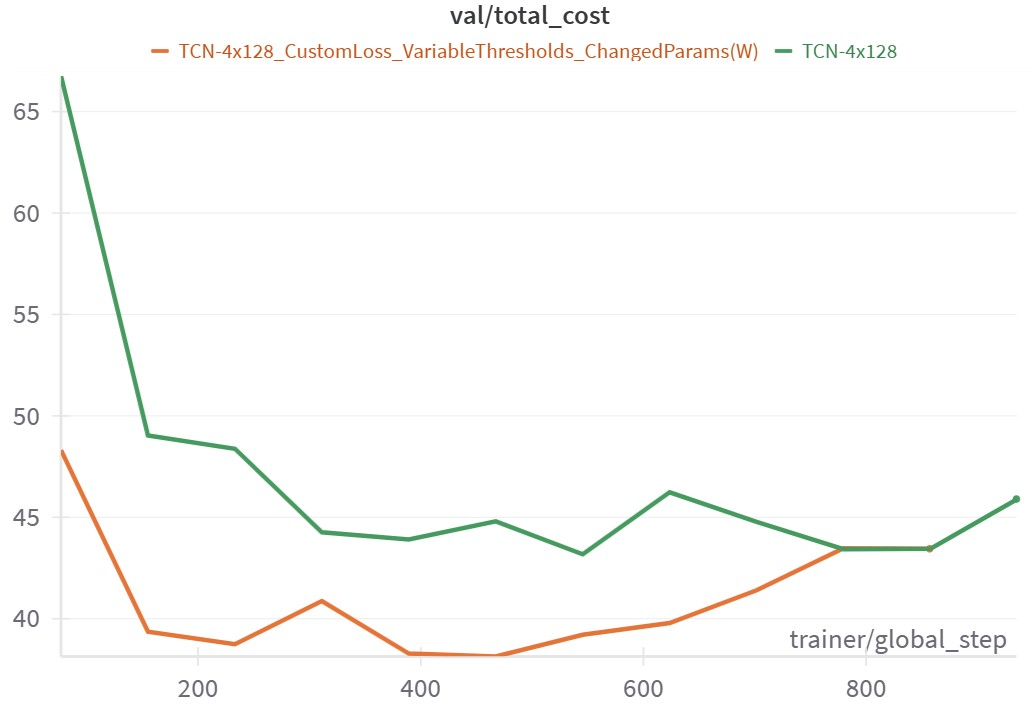
\includegraphics[width=0.8\textwidth]{figs/Total Validation Cost Comparison.jpg}
    \caption{Total validation cost comparison between base TCN and TCN with applied improvement strategies on the validation set.}
    \label{fig:Total Validation Cost Comparison}
\end{figure}

So we decided on the mentioned combination for our final model. This model now yields an unbiased cost estimate on the test dataset of 41.038 \footnote{Additional improvement strategies were explored, as can be seen in the following link: \url{https://wandb.ai/mlpc2025/mlpc2025_challenge?nw=nwusertylernavarro}.}

We then retrained our final model on the entirety of the provided data for 6 epochs (as the optimum for the best model on the validation data was achieved after 6 epochs) in order to create our predictions for the secret customer test set, utilizing the thresholds determined by the model trained on less of the data.



\newpage


\section{Do you think your final system could be deployed in a real-world application?}
\label{sec:real-world application}


The question of whether our system could be deployed in a real-world application is not trivial and depends heavily on the specific use case. However, generally speaking, in our opinion, the current version of our system cannot be used as-is in a real world setting. This is primarily due to three reasons:

1) Mismatch between Training Data and Real World Conditions
The recordings we used in our dataset were collected from a publicly available source and created by individuals with no specific use case in mind. This means that important factors like sound/recording quality and individual sound events will almost certainly differ between our dataset and a real-world setting. As a result, the network is not trained for its actual task. Additionally, the predicted accuracy—based on our test set—will likely be highly overoptimistic.

2) Lack of Task specific Data
The dataset was intentionally designed to be very general, which is beneficial for research but a weakness when it comes to real-world application. Depending on the task, the model would likely have to make more distinct differentiations (e.g., a car starting vs. a car driving vs. a car stopping), while other samples may not be needed at all—like the sound of a bee, when dealing with neighborhood noise infractions (I don't want to meet the bee that can rival a car's volume).

3) Risk of Implicit Bias in the Text Annotations
The annotations for the dataset were created by a group of people with very similar cultural backgrounds. This almost certainly introduces several biases. In real-world settings, sound perception can differ significantly between individuals, which would affect the system’s usefulness.



If we want to implement our system in a real-world application, we would have to make some changes. The main issue lies with the dataset. Assuming we want our model to perform as well as it can, we would need to collect data in the same way we expect future, unseen data to be recorded—preferably even at a similar location.\n

Furthermore, our model would benefit from more refined sample selection. Eliminating unnecessary classes and adding more nuanced, region specific ones.

\n Lastly, we should consider involving a more diverse group of data engineers to label the training data, to minimize the risks of implicit bias.

\n

Overall our system is a solid foundation on which more use case specific model could be trained.


\subsection{In your opinion, which aspects of the project or your system would need to be adapted to fulfill possible real-world requirements?}
\label{sec:real-world-app:a}





\newpage


\section{Bonus}
\label{sec:Bonus}

So far, we’ve worked with audio embeddings, that were created from a pre-trained and frozen sound event detection model. 
To receive the bonus points, train one of our pre-trained sound event detection models on the MLPC dataset to predict the ten sound categories of interest in an end-to-end manner. 
You can find an implementation, a detailed documentation and pre-trained checkpoints here: \url{https://github.com/fschmid56/PretrainedSED} . 
Use one of the checkpoint that was pre-trained on AudioSet-strong as a starting point. 
You can use any of the model architectures. 
Compare the performance of the resulting system to the best model from the previous section.



\subsection{Train one of our pre-trained sound event detection models on the MLPC dataset to predict the ten sound categories of interest in an end-to-end manner.}
\label{sec:Bonus:a}

\begin{figure}[htbp]
    \centering
    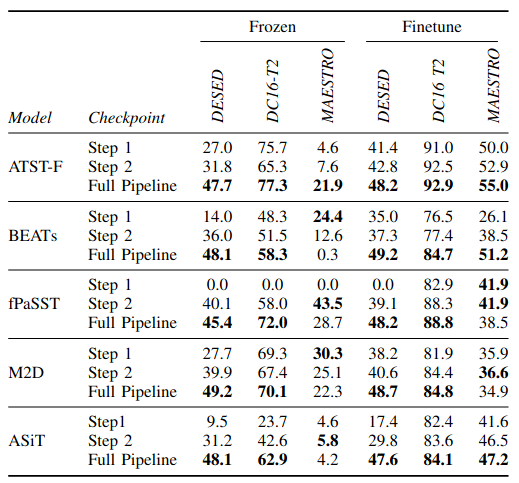
\includegraphics[width=0.4\textwidth]{figs/downstream_task_results.png}
    \caption{Downstream Task Performances}
    \label{fig:Downstream Task Performances}
\end{figure}



\subsection{You can use any of the model architectures.}
\label{sec:Bonus:b}

We wanted to use a Transformer model as we haven't tested it yet. Due to the downstream task performance (Figure~\ref{fig:Downstream Task Performances}), we decided on the model ATST-F (./models/atstframe).
\newline
We used the Pre-Trained Model Checkpoint from here: 
\newline

\url{https://github.com/fschmid56/PretrainedSED/releases/download/v0.0.1/ATST-F_strong_1.pt} .



\subsection{Compare the performance of the resulting system to the best model from the previous section.}
\label{sec:Bonus:c}






\end{document}
